\documentclass{article}

\RequirePackage[svgnames]{xcolor}
\definecolor{UTorange}{RGB}{207, 83, 0} 
\definecolor{UTwhite}{RGB}{214, 210, 196}
\definecolor{UTgray}{RGB}{51, 63, 72}

\definecolor{UCLAblue}{RGB}{39, 116, 174} 
\definecolor{UCLAdark}{RGB}{0, 59, 92}
\definecolor{UCLAlight}{RGB}{218, 235, 254}
\definecolor{UCLAgold}{RGB}{255, 209, 0}

\definecolor{mered}{HTML}{882255}
\definecolor{megreen}{HTML}{004953}
\definecolor{mepink}{HTML}{AA4499}
\definecolor{rosequartz}{HTML}{F7CAC9}
\definecolor{serenity}{HTML}{92A8D1}

\definecolor{dark-red}{rgb}{0.4,0.15,0.15}
\definecolor{dark-blue}{rgb}{0.15,0.15,0.4}
\definecolor{medium-blue}{rgb}{0,0,0.5}

\usepackage{amsmath,amssymb, enumerate, tikz-cd,mathrsfs,hyperref,colortbl,bm}
\usepackage{graphicx, animate,lmodern}
\usepackage[export]{adjustbox}
\usepackage{cleveref}



%\usepgfplotslibrary{external}
 % \usetikzlibrary{external}
 % \tikzexternalize[prefix=tikz/]

\usepackage{float}
\usepackage{caption}
\usepackage{tikz}
\usepackage{tikz-3dplot}
\usepackage{pgfplots}
\pgfplotsset{compat=1.18}
\usetikzlibrary{scopes, angles, quotes, arrows.meta, calc, positioning}


\newcommand\fixthis[1]{\textcolor{red}{#1}}

\newcommand{\R}{\mathbb{R}}
\newcommand{\C}{\mathbb{C}}
\newcommand{\Z}{\mathbb{Z}}
\newcommand{\Q}{\mathbb{Q}}
\newcommand{\F}{\mathbb{F}}
\newcommand{\N}{\mathbb{N}}

%my macros
\newcommand{\Sphere}{\mathbb{S}}
\newcommand{\TatekG}{\mathsf{Tate}(kG)}
\newcommand{\kGMod}{kG$-$\mathsf{Mod}}
\newcommand{\StMod}{\mathsf{StMod}}
\newcommand{\Mod}{\mathsf{Mod}}
\newcommand{\Top}{\textnormal{Top}}
\newcommand{\D}{\mathcal{D}}
\newcommand{\Ho}{\mathsf{Ho}}
\newcommand{\Hom}{\textnormal{Hom}}
\newcommand{\Ext}{\textnormal{Ext}}
\newcommand{\Tor}{\textnormal{Tor}}
\newcommand{\Cell}{\mathsf{Cell}}
\newcommand{\End}{\mathsf{End}}
\newcommand{\Spec}{\textnormal{Spec}}
\newcommand{\holim}{\textnormal{holim}}
\newcommand{\hocolim}{\textnormal{hocolim}}
\newcommand{\1}{\mathds{1}}
\newcommand{\Supp}{\textnormal{Supp}}
\newcommand{\supp}{\textnormal{supp}}
\newcommand{\Pic}{\textnormal{Pic}}
\newcommand{\pic}{\mathfrak{pic}}
\newcommand{\gl}{\mathfrak{gl}}
\newcommand{\Tot}{\textnormal{Tot}}
\newcommand{\CAlg}{\textnormal{CAlg}}
\newcommand{\Res}{\textnormal{Res}}
\newcommand{\CoInd}{\textnormal{CoInd}}


\begin{document}
	
	
	\begin{center}
		\begin{tikzpicture}[x=1cm, y=1cm, z=-0.6cm, scale=0.5]
			% Axes
			\draw [<->] (-4,0,0) -- (4,0,0) node [right] {};
			
			% Ticks
			\foreach \i in {-3,-2, -1, 0, 1,2,3}
			{
				\draw (\i,-0.1,0) -- ++ (0,0.2,0);
			}
			
		\end{tikzpicture}
	\end{center}
	
	
	\begin{center}
		\begin{center}\begin{tikzpicture}[scale=.65]
				\pgfmathsetmacro{\entrya}{3}
				\pgfmathsetmacro{\entryb}{2}
				\clip (-3,-3) rectangle (3,3);
				% Axes
				\draw [<->] (-3,0) -- (3,0) node [below left] {$x$};
				\draw [<->] (0,-3) -- (0,3) node [below right] {$y$};
				
				% Ticks
				\foreach \i in {-2, -1, 0, 1,2}
				{
					\draw (-0.1,\i) -- ++ (0.2,0);
					\draw (\i,-0.1) -- ++ (0,0.2);
				}
				
			\end{tikzpicture}
		\end{center}
	\end{center}
	
	\begin{center}
		\begin{tikzpicture}[x=1cm, y=1cm, z=-0.6cm, scale=0.5]
			\pgfmathsetmacro{\cubex}{3}
			\pgfmathsetmacro{\cubey}{2.5}
			\pgfmathsetmacro{\cubez}{3.14}
			% Axes
			\draw [<->] (-4,0,0) -- (4,0,0) node [right] {$y$};
			\draw [<->] (0,-4,0) -- (0,4,0) node [left] {$z$};
			\draw [<->] (0,0,-4) -- (0,0,4) node [left] {$x$};
			
			% Ticks
			\foreach \i in {-3,-2, -1, 0, 1,2,3}
			{
				\draw (-0.1,\i,0) -- ++ (0.2,0,0);
				\draw (\i,-0.1,0) -- ++ (0,0.2,0);
				\draw (-0.1,0,\i) -- ++ (0.2,0,0);
			}
			
		\end{tikzpicture}
	\end{center}

%  \tdplotsetmaincoords{60}{110}
% \begin{tikzpicture}[scale=3, tdplot_main_coords]
%     \coordinate (O) at (0,0,0);
%     \draw[thick,->] (0,0,0) -- (1,0,0) node[anchor=north east]{$x$};
%     \draw[thick,->] (0,0,0) -- (0,1,0) node[anchor=north west]{$y$};
%     \draw[thick,->] (0,0,0) -- (0,0,1) node[anchor=south]{$z$};
%     \tdplotsetcoord{P}{1}{30}{60}
%     \draw plot [mark=*, mark size=0.2] (P) node [right] {\scriptsize$(x,y,z)$}; 
%     \draw[dashed] (O) -- (P);
%     \draw[dashed, color=black] (O) -- (Pxy);
%     \draw[dashed, color=black] (P) -- (Pxy);
%     \draw[dashed, color=black] (P) -- (Pz) node [below left] {$z$};
%     \draw[dashed, color=black] (Pxy) -- (Px) node [left] {$x$};
%     \draw[dashed, color=black] (Pxy) -- (Py) node [above] {$y$};
% \end{tikzpicture}
	
	\begin{center}
		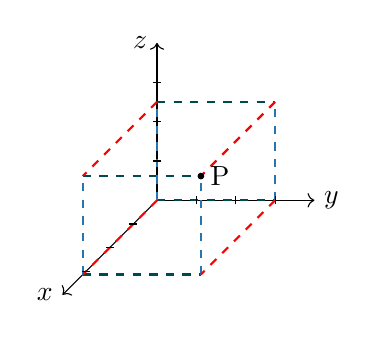
\begin{tikzpicture}[x=1cm, y=1cm, z=-0.6cm, scale=0.5]
			\pgfmathsetmacro{\cubex}{3}
			\pgfmathsetmacro{\cubey}{2.5}
			\pgfmathsetmacro{\cubez}{3.14}
			% Axes
			\draw [->] (0,0,0) -- (4,0,0) node [right] {$y$};
			\draw [->] (0,0,0) -- (0,4,0) node [left] {$z$};
			\draw [->] (0,0,0) -- (0,0,4) node [left] {$x$};
			
			\draw[megreen,dashed, thick] (0,0,0) -- (\cubex,0,0);
			\draw[megreen,dashed, thick] (0,\cubey,0) -- (\cubex,\cubey,0);
			\draw[megreen,dashed, thick] (0,0,\cubez) -- (\cubex,0,\cubez);
			\draw[megreen,dashed, thick] (0,\cubey,\cubez) -- (\cubex,\cubey,\cubez);
			
			\draw[UCLAblue,dashed, thick] (0,0,0) -- (0,\cubey,0);
			\draw[UCLAblue,dashed, thick] (\cubex,0,0) -- (\cubex,\cubey,0);
			\draw[UCLAblue,dashed, thick] (0,0,\cubez) -- (0,\cubey,\cubez);
			\draw[UCLAblue,dashed, thick] (\cubex,0,\cubez) -- (\cubex,\cubey,\cubez);
			
			\draw[red,dashed, thick] (0,0,0) -- (0,0,\cubez);
			\draw[red,dashed, thick] (\cubex,0,0) -- (\cubex,0,\cubez);
			\draw[red,dashed, thick] (0,\cubey,0) -- (0,\cubey,\cubez);
			\draw[red,dashed, thick] (\cubex,\cubey,0) -- (\cubex,\cubey,\cubez);
			
			\filldraw[black] (\cubex,\cubey,\cubez) circle (2pt) node[anchor=west]{P};
			% % Vectors
			% \draw [->, thick] (0,0,0) -- (2,2,0);
			% \draw [->, thick] (0,0,0) -- (2,0,1);
			% Ticks
			\foreach \i in {1,2,3}
			{
				\draw (-0.1,\i,0) -- ++ (0.2,0,0);
				\draw (\i,-0.1,0) -- ++ (0,0.2,0);
				\draw (-0.1,0,\i) -- ++ (0.2,0,0);
			}
			
		\end{tikzpicture}
	\end{center}
	
	\begin{center}
		\begin{tikzpicture}[x=1cm, y=1cm, z=-0.6cm, scale=0.5]
			\pgfmathsetmacro{\cubex}{0}
			\pgfmathsetmacro{\cubey}{3.14}
			\pgfmathsetmacro{\cubez}{3}
			\pgfmathsetmacro{\cubexx}{3}
			\pgfmathsetmacro{\cubeyy}{2.72}
			\pgfmathsetmacro{\cubezz}{4}
			% Axes
			\draw [->] (0,0,0) -- (4,0,0) node [right] {$y$};
			\draw [->] (0,0,0) -- (0,4,0) node [left] {$z$};
			\draw [->] (0,0,0) -- (0,0,4) node [left] {$x$};
			
			\draw[UCLAblue, thick, -Latex] (\cubex,\cubey,\cubez) -- (\cubexx,\cubeyy,\cubezz);
			
			\filldraw[black] (\cubex,\cubey,\cubez) circle (2pt) node[anchor=west]{P};
			\filldraw[black] (\cubexx,\cubeyy,\cubezz) circle (2pt) node[anchor=west]{Q};
			% % Vectors
			% \draw [->, thick] (0,0,0) -- (2,2,0);
			% \draw [->, thick] (0,0,0) -- (2,0,1);
			% Ticks
			\foreach \i in {1,2,3}
			{
				\draw (-0.1,\i,0) -- ++ (0.2,0,0);
				\draw (\i,-0.1,0) -- ++ (0,0.2,0);
				\draw (-0.1,0,\i) -- ++ (0.2,0,0);
			}
			
		\end{tikzpicture}
	\end{center}
	
	
	\begin{center}
		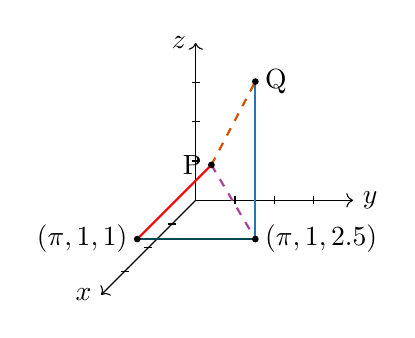
\begin{tikzpicture}[x=1cm, y=1cm, z=-0.6cm, scale=0.5]
			\pgfmathsetmacro{\cubex}{3}
			\pgfmathsetmacro{\cubey}{4}
			\pgfmathsetmacro{\cubez}{3.14}
			% Axes
			\draw [->] (0,0,0) -- (4,0,0) node [right] {$y$};
			\draw [->] (0,0,0) -- (0,4,0) node [left] {$z$};
			\draw [->] (0,0,0) -- (0,0,4) node [left] {$x$};
			
			\draw[red, thick] (1,1.5,1) -- (1,1.5,\cubez+1);
			\draw[megreen, thick] (1,1.5,\cubez+1) -- (\cubex+1,1.5,\cubez+1);
			\draw[UCLAblue, thick] (\cubex+1,1.5,\cubez+1) -- (\cubex+1,\cubey+1.5,\cubez+1);
			
			\draw[mepink,dashed, thick](1,1.5,1) -- (\cubex+1,1.5,\cubez+1);
			\draw[UTorange,dashed, thick] (1,1.5,1) -- (\cubex+1,\cubey+1.5,\cubez+1);
			
			\filldraw[black] (1,1.5,\cubez+1) circle (2pt) node[anchor=east]{$(\pi, 1, 1)$};
			\filldraw[black] (\cubex+1,1.5,\cubez+1) circle (2pt) node[anchor=west]{$(\pi, 1, 2.5)$};
			\filldraw[black] (\cubex+1,\cubey+1.5,\cubez+1) circle (2pt) node[anchor=west]{Q};
			\filldraw[black] (1,1.5,1) circle (2pt) node[anchor=east]{P};
			% % Vectors
			% \draw [->, thick] (0,0,0) -- (2,2,0);
			% \draw [->, thick] (0,0,0) -- (2,0,1);
			% Ticks
			\foreach \i in {1,2,3}
			{
				\draw (-0.1,\i,0) -- ++ (0.2,0,0);
				\draw (\i,-0.1,0) -- ++ (0,0.2,0);
				\draw (-0.1,0,\i) -- ++ (0.2,0,0);
			}
			
		\end{tikzpicture}
	\end{center}
	
	
	\begin{center}
		\begin{tikzpicture}[x=1cm, y=1cm, z=-0.6cm, scale=0.5]
			
			% Axes
			\draw [->] (0,0,0) -- (4,0,0) node [right] {$y$};
			\draw [->] (0,0,0) -- (0,4,0) node [left] {$z$};
			\draw [->] (0,0,0) -- (0,0,4) node [left] {$x$};
			
			\draw[red, thick, -Latex] (0,0,0) -- (0,0,1) node [left] {$\bm{i}$};
			\draw[megreen, thick, -Latex] (0,0,0) -- (0,1,0) node [right]{$\bm{k}$};
			\draw[UCLAblue, thick, -Latex] (0,0,0) -- (1,0,0) node [below] {$\bm{j}$};
			
			% % Vectors
			% \draw [->, thick] (0,0,0) -- (2,2,0);
			% \draw [->, thick] (0,0,0) -- (2,0,1);
			% Ticks
			\foreach \i in {1,2,3}
			{
				\draw (-0.1,\i,0) -- ++ (0.2,0,0);
				\draw (\i,-0.1,0) -- ++ (0,0.2,0);
				\draw (-0.1,0,\i) -- ++ (0.2,0,0);
			}
			
		\end{tikzpicture}
	\end{center}
	
	
	
	\begin{center}
		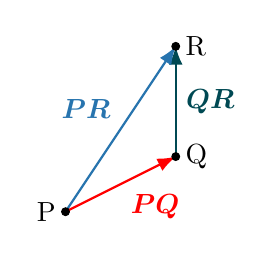
\begin{tikzpicture}[scale=0.7]
			\pgfmathsetmacro{\cubex}{2}
			\pgfmathsetmacro{\cubey}{3}
			
			
			
			\draw[red, thick, -Latex] (0,0) -- (\cubex,1) node[midway,below right] {$\bm{PQ}$};
			\draw[megreen, thick, -Latex] (\cubex,1) -- (\cubex,\cubey) node[midway, right] {$\bm{QR}$};
			\draw[UCLAblue, thick, -Latex] (0,0) -- (\cubex,\cubey) node[midway,above left] {$\bm{PR}$};
			
			
			\filldraw[black] (0,0) circle (2pt) node[anchor=east]{P};
			\filldraw[black] (\cubex,1) circle (2pt) node[anchor=west]{Q};
			\filldraw[black] (\cubex,\cubey) circle (2pt) node[anchor=west]{R};
			
		\end{tikzpicture}
	\end{center}
	
	
	\begin{center}
		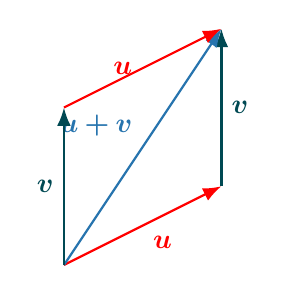
\begin{tikzpicture}scale=0.5]
			\pgfmathsetmacro{\cubex}{2}
			\pgfmathsetmacro{\cubey}{3}
			
			
			
			\draw[red, thick, -Latex] (0,0) -- (\cubex,1) node[midway,below right] {$\bm{u}$};
			\draw[megreen, thick, -Latex] (\cubex,1) -- (\cubex,\cubey) node[midway, right] {$\bm{v}$};
			\draw[UCLAblue, thick, -Latex] (0,0) -- (\cubex,\cubey) node[midway,above left] {$\bm{u+v}$};
			\draw[megreen, thick, -Latex] (0,0) -- (0,\cubey-1) node[midway,left] {$\bm{v}$};
			\draw[red, thick, -Latex] (0, \cubey-1) -- (\cubex,\cubey) node[midway,left] {$\bm{u}$};
			
			
			
		\end{tikzpicture}
	\end{center}
	
	
	\begin{center}
		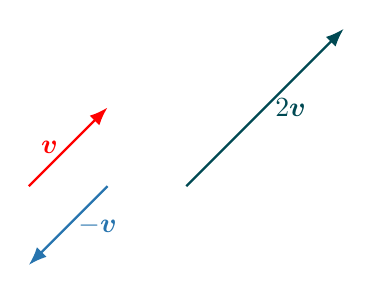
\begin{tikzpicture}scale=0.5]
			\pgfmathsetmacro{\cubex}{1}
			\pgfmathsetmacro{\cubey}{3}
			
			
			
			\draw[red, thick, -Latex] (-1,0) -- (-1+\cubex,\cubex) node[midway, left] {$\bm{v}$};
			\draw[megreen, thick, -Latex] (1,0) -- (2*\cubex+1,2*\cubex) node[midway, right] {$2\bm{v}$};
			\draw[UCLAblue, thick, -Latex] (0,0) -- (-\cubex,-\cubex) node[midway, right] {$-\bm{v}$};
			
			
			
		\end{tikzpicture}
	\end{center}
	
	
	
	
	\begin{center}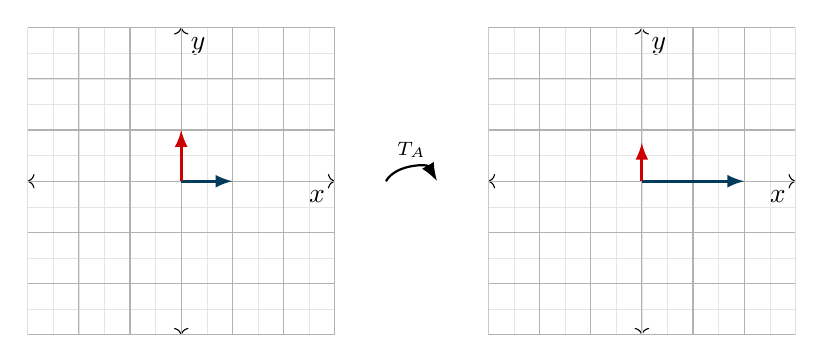
\begin{tikzpicture}[scale=.65]
			
			\begin{scope}
				\clip (-3,-3) rectangle (3,3);
				% Axes
				\draw [<->] (-3,0) -- (3,0) node [below left] {$x$};
				\draw [<->] (0,-3) -- (0,3) node [below right] {$y$};
				%grid
				\draw[step=0.5cm, gray!20!white, very thin] (-3,-3) grid (3,3);
				\draw[step=1cm, gray!60!white, thin] (-3,-3) grid (3,3);
				
				\draw[color=UCLAdark, line width=1.10pt, -latex] (0, 0) -- (1,0);
				\draw[color=red!80!black, line width=1.10pt, -latex] (0, 0) -- (0,1);
				
			\end{scope}
			
			\begin{scope}[xshift=9cm]
				%all you need to change are the entries in the matrix using the following 4 macros
				\pgfmathsetmacro{\entrya}{2}
				\pgfmathsetmacro{\entryb}{0}
				\pgfmathsetmacro{\entryc}{0}
				\pgfmathsetmacro{\entryd}{.75}
				
				
				\clip (-3,-3) rectangle (3,3);
				% Axes
				\draw [<->] (-3,0) -- (3,0) node [below left] {$x$};
				\draw [<->] (0,-3) -- (0,3) node [below right] {$y$};
				%grid
				\draw[step=0.5cm, gray!20!white, very thin] (-3,-3) grid ((3,3);
				\draw[step=1cm, gray!60!white, thin] (-3,-3) grid (3,3);
				
				% \foreach \x in {-5,...,5} {
				% \draw[domain=-3:3,smooth,variable=\t,color=UCLAblue, thick]plot (\entrya*\t+\x*\entryb,\entryc*\t+\x*\entryd);
				% }
				
				% \foreach \y in {-5,...,5} {
				% \draw[domain=-3:3,smooth,variable=\t,color=mered, thick]plot (\entryb*\t+\y*\entrya,\entryd*\t+\y*\entryc);
				% }
				
				
				\draw[color=UCLAdark, line width=1.10pt, -latex] (0, 0) -- (\entrya, \entryc);
				\draw[color=red!80!black, line width=1.10pt, -latex] (0, 0) -- (\entryb, \entryd);
			\end{scope}
			
			
			
			\draw[thick,-Latex] (4,0) to[out=60,in=120] node[midway,font=\scriptsize,above] {$T_A$} (5,0);
			
		\end{tikzpicture}
	\end{center}
	
	\begin{center}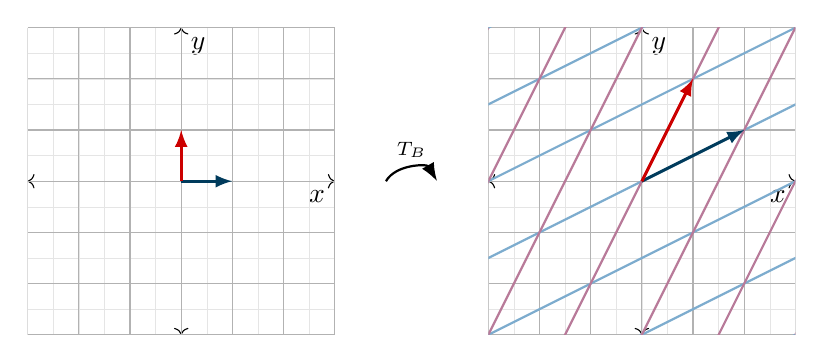
\begin{tikzpicture}[scale=.65]
			
			\begin{scope}
				\clip (-3,-3) rectangle (3,3);
				% Axes
				\draw [<->] (-3,0) -- (3,0) node [below left] {$x$};
				\draw [<->] (0,-3) -- (0,3) node [below right] {$y$};
				%grid
				\draw[step=0.5cm, gray!20!white, very thin] (-3,-3) grid (3,3);
				\draw[step=1cm, gray!60!white, thin] (-3,-3) grid (3,3);
				
				\draw[color=UCLAdark, line width=1.10pt, -latex] (0, 0) -- (1,0);
				\draw[color=red!80!black, line width=1.10pt, -latex] (0, 0) -- (0,1);
				
			\end{scope}
			
			\begin{scope}[xshift=9cm]
				%all you need to change are the entries in the matrix using the following 4 macros
				\pgfmathsetmacro{\entrya}{2}
				\pgfmathsetmacro{\entryb}{1}
				\pgfmathsetmacro{\entryc}{1}
				\pgfmathsetmacro{\entryd}{2}
				
				
				\clip (-3,-3) rectangle (3,3);
				% Axes
				\draw [<->] (-3,0) -- (3,0) node [below left] {$x$};
				\draw [<->] (0,-3) -- (0,3) node [below right] {$y$};
				%grid
				\draw[step=0.5cm, gray!20!white, very thin] (-3,-3) grid (3,3);
				\draw[step=1cm, gray!60!white, thin] (-3,-3) grid (3,3);
				
				\foreach \x in {-5,...,5} {
					\draw[domain=-3:3,smooth,variable=\t,color=UCLAblue!60!white, thick]plot (\entrya*\t+\x*\entryb,\entryc*\t+\x*\entryd);
				}
				
				\foreach \y in {-5,...,5} {
					\draw[domain=-3:3,smooth,variable=\t,color=mered!60!white, thick]plot (\entryb*\t+\y*\entrya,\entryd*\t+\y*\entryc);
				}
				
				
				\draw[color=UCLAdark, line width=1.10pt, -latex] (0, 0) -- (\entrya, \entryc);
				\draw[color=red!80!black, line width=1.10pt, -latex] (0, 0) -- (\entryb, \entryd);
			\end{scope}
			
			
			
			\draw[thick,-Latex] (4,0) to[out=60,in=120] node[midway,font=\scriptsize,above] {$T_B$} (5,0);
			
		\end{tikzpicture}
	\end{center}
	
	
	
	\begin{center}
		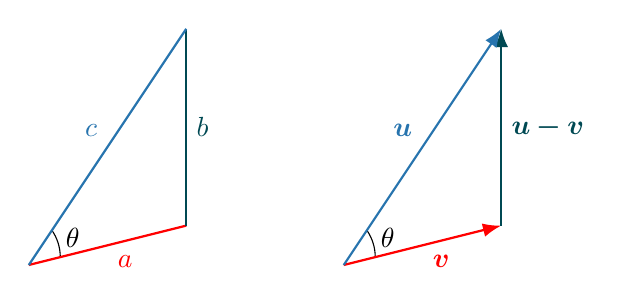
\begin{tikzpicture}
			\begin{scope}
				\pgfmathsetmacro{\cubex}{2}
				\pgfmathsetmacro{\cubey}{3}
				
				
				\draw (0.4,0.1) arc [start angle=0,end angle=35,radius=0.6] node[pos=0.7,right]{$\theta$};
				\draw[red, thick] (0,0) -- (\cubex,0.5) node[midway,below right] {$a$};
				\draw[megreen, thick] (\cubex,0.5) -- (\cubex,\cubey) node[midway, right] {$b$};
				\draw[UCLAblue, thick] (0,0) -- (\cubex,\cubey) node[midway,above left] {$c$};
				
			\end{scope}
			
			\begin{scope}[xshift=4cm]
				\pgfmathsetmacro{\cubex}{2}
				\pgfmathsetmacro{\cubey}{3}
				
				
				\draw (0.4,0.1) arc [start angle=0,end angle=35,radius=0.6] node[pos=0.7, right]{$\theta$};
				\draw[red, thick, -Latex] (0,0) -- (\cubex,0.5) node[midway,below right] {$\bm{v}$};
				\draw[megreen, thick, -Latex] (\cubex,0.5) -- (\cubex,\cubey) node[midway, right] {$\bm{u-v}$};
				\draw[UCLAblue, thick, -Latex] (0,0) -- (\cubex,\cubey) node[midway,above left] {$\bm{u}$};
				
			\end{scope}
		\end{tikzpicture}
	\end{center}
	
	\begin{center}
		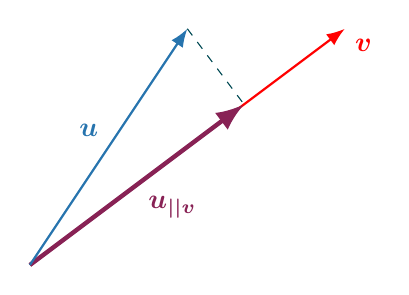
\begin{tikzpicture}scale=0.5]
			\pgfmathsetmacro{\cubex}{2}
			\pgfmathsetmacro{\cubey}{3}
			
			
			\draw[megreen, dashed] (\cubex,\cubey) -- (2.72, 2.04);
			\draw[red, thick, -Latex] (0,0) -- (4,3) node[below right] {$\bm{v}$};
			\draw[mered, ultra thick, -Latex] (0,0) -- (2.72, 2.04) node[midway,below right] {$\bm{u_{||v}}$};
			\draw[UCLAblue, thick, -Latex] (0,0) -- (\cubex,\cubey) node[midway,above left] {$\bm{u}$};
			
			
			
		\end{tikzpicture}
	\end{center}    
	
	
	\begin{center}
		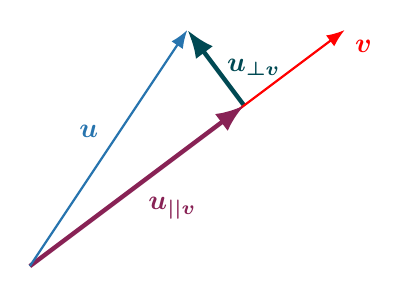
\begin{tikzpicture}scale=0.5]
			\pgfmathsetmacro{\cubex}{2}
			\pgfmathsetmacro{\cubey}{3}
			
			
			\draw[megreen, ultra thick, -Latex] (2.72, 2.04) -- (\cubex,\cubey)  node[midway, right] {$\bm{u_{\bot v}}$};
			\draw[red, thick, -Latex] (0,0) -- (4,3) node[below right] {$\bm{v}$};
			\draw[mered, ultra thick, -Latex] (0,0) -- (2.72, 2.04) node[midway,below right] {$\bm{u_{||v}}$};
			\draw[UCLAblue, thick, -Latex] (0,0) -- (\cubex,\cubey) node[midway,above left] {$\bm{u}$};
			
			
			
		\end{tikzpicture}
	\end{center}    
	
	\begin{center}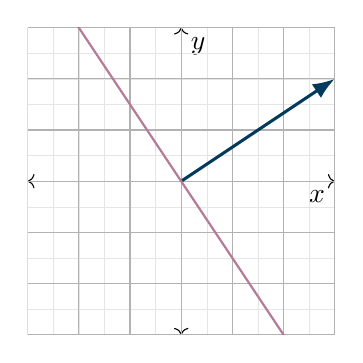
\begin{tikzpicture}[scale=.65]
			\pgfmathsetmacro{\entrya}{3}
			\pgfmathsetmacro{\entryb}{2}
			\clip (-3,-3) rectangle (3,3);
			% Axes
			\draw [<->] (-3,0) -- (3,0) node [below left] {$x$};
			\draw [<->] (0,-3) -- (0,3) node [below right] {$y$};
			%grid
			\draw[step=0.5cm, gray!20!white, very thin] (-3,-3) grid (3,3);
			\draw[step=1cm, gray!60!white, thin] (-3,-3) grid (3,3);
			
			\draw[color=UCLAdark, line width=1.10pt, -Latex] (0, 0) -- (\entrya,\entryb);
			
			\draw[domain=-3:3,smooth,variable=\t,color=mered!60!white, thick]plot (\entryb*\t,-\entrya*\t);
			
			
		\end{tikzpicture}
	\end{center}
	
	
	\begin{center}
		\tdplotsetmaincoords{105}{-30}
		\begin{tikzpicture}[tdplot_main_coords,scale=.5]
			\tdplotsetrotatedcoords{00}{30}{0}
			\begin{scope}[tdplot_rotated_coords]
				\begin{scope}[canvas is xy plane at z=0]
					\fill[gray,fill opacity=0.3] (-2,-3) rectangle (2,3); 
					\pgflowlevelsynccm
				\end{scope} 
				\draw[very thick,-Latex,color=UCLAdark] (0,0,0) coordinate (O) -- (0,0,3) node[right]{$\bm{n}$};
			\end{scope}
			\pgfmathsetmacro{\Radius}{1.5}
			\draw[-stealth]  (O)-- (2.5*\Radius,0,0) node[pos=1.15] {$y$};
			\draw[-stealth] (O) -- (0,3.5*\Radius,0) node[pos=1.15] {$x$};
			\draw[-stealth] (O) -- (0,0,2.5*\Radius) node[pos=1.05] {$z$};
		\end{tikzpicture} 
	\end{center}
	
	
	\begin{center}
		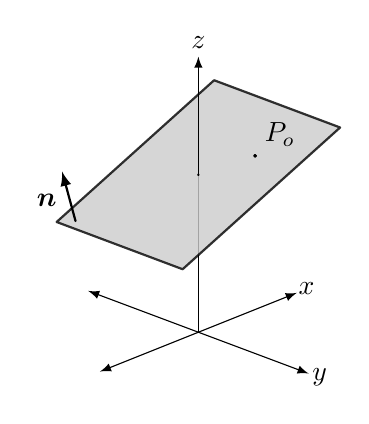
\begin{tikzpicture}[x={(1cm,0.4cm)}, y={(8mm, -3mm)}, z={(0cm,1cm)}, line cap=round, line join=round, scale=0.5]
			\def\t{0.9}
			\def\s{0.04}
			\def\tt{0.3}
			\def\ss{0.7}
			\def\ttt{0.5}
			\def\sss{0.5}
			%Coordinates
			%Plane Vertex Points
			\coordinate (x1) at (-2,2,3);
			\coordinate (x2) at (2,2,5);
			\coordinate (x3) at (2,-2,5);
			\coordinate (x4) at (-2,-2,3);
			%Vectors Parallel to Plane
			\coordinate (n1) at ($(x2) - (x1)$);
			\coordinate (n2) at ($(x2) - (x3)$); 
			%Points on Plane
			\coordinate (x5) at ($(x1) + \s*(n1) - \t*(n2)$);
			\node[outer sep = 1pt, inner sep = 1pt] (x6) at ($(x1) + \ss*(n1) - \tt*(n2)$) {};
			\coordinate (x7) at ($(x1) + \sss*(n1) - \ttt*(n2)$);
			%Beginning of Axis
			\coordinate (O) at (0,0,0);
			%Random Point
			\node[outer sep = 1pt, inner sep = 1pt] (P) at (2.5,1,5.5) {};
			
			%Axis 	
			\draw[latex-latex] (-2.5,0,0) -- (2.5,0,0) node[pos = 1.05] {$x$};
			\draw[latex-latex] (0,-3.5,0) -- (0,3.5,0) node[pos = 1.05] {$y$};
			\draw[-latex] (0,0,0) -- (0,0,7) node[pos = 1.05] {$z$};
			%\draw[draw=black, fill=black] (O) circle (1pt) node[below] {${O}$};
			
			%Point on Plane
			%\draw[-latex, thick] (O) -- (x6) node[pos=0.45, shift={(0.1,0.3)}] {$\vb{r_o}$};
			%Plane
			\path[draw=black, fill=black!20, thick, opacity = 0.8] (x1) -- (x2) -- (x3) -- (x4) -- (x1);
			%\node[shift={(-0.45,0.6)}] at (x3) {$P$};
			%Perpendicular Vector
			\draw[-latex, thick] (x5) -- ($(x5)!0.07!(-8,0,24)$) node[pos=0.5, shift={(-0.2,-0.1)}] {$\bm{n}$};
			%Point on Plane	
			\draw[draw=black, fill=black] (x6) circle (1pt) node[above right] {${P_o}$};
			
			%Z-axis Section
			\draw[draw=black, fill=black] (x7) circle (0.5pt);
			\draw (x7) -- (0,0,6.5);
			
			%	%Random Point
			%	\draw[-latex, thick] (O) -- (P) node[pos=0.45, shift={(0.1,0.3)}] {$\vb{r}$};
			%	\draw[draw=black, fill=black] (P) circle (1pt) node[above right] {$\mathrm{P}$};
			
		\end{tikzpicture}
	\end{center}
	
	\begin{center}
		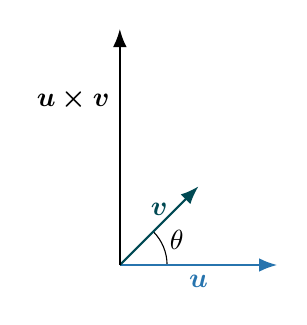
\begin{tikzpicture}
			\draw (0.6,0) arc [start angle=0,end angle=45,radius=0.6]
			node[pos=0.7,right]{$\theta$};
			\draw[thick,-Latex,UCLAblue](0,0)--(2,0)node[midway,below]{$\bm{u}$};
			\draw[thick,-Latex,megreen](0,0)--(1,1)node[midway,above]{$\bm{v}$};
			\draw[thick,-Latex,](0,0)--(0,3)node[pos=0.7,left]{$\bm{u \times v}$};
		\end{tikzpicture}
	\end{center}
	
	\begin{center}
		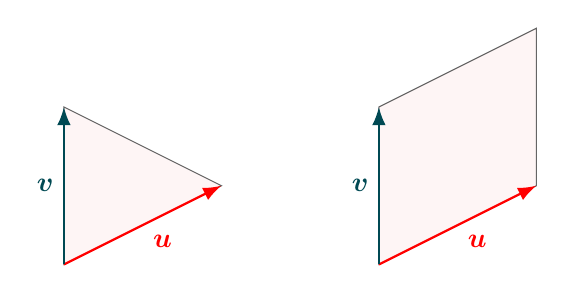
\begin{tikzpicture}scale=0.5]
			\begin{scope}
				\pgfmathsetmacro{\cubex}{2}
				\pgfmathsetmacro{\cubey}{3}
				
				
				\draw[fill=rosequartz!30,opacity=0.6] (0,0) -- (\cubex,1) -- (0,\cubey-1) -- cycle;
				
				\draw[red, thick, -Latex] (0,0) -- (\cubex,1) node[midway,below right] {$\bm{u}$};
				\draw[megreen, thick, -Latex] (0,0) -- (0,\cubey-1) node[midway, left] {$\bm{v}$};
				
				
			\end{scope}
			
			\begin{scope}[xshift=4cm]
				
				\pgfmathsetmacro{\cubex}{2}
				\pgfmathsetmacro{\cubey}{3}
				
				\draw[fill=rosequartz!30,opacity=0.6] (0,0) -- (\cubex,1)  -- (\cubex,\cubey) -- (0,\cubey-1)-- cycle;
				
				\draw[red, thick, -Latex] (0,0) -- (\cubex,1) node[midway,below right] {$\bm{u}$};
				\draw[megreen, thick, -Latex] (0,0) -- (0,\cubey-1) node[midway,left] {$\bm{v}$};
				
			\end{scope}
			
			
			
			
		\end{tikzpicture}
	\end{center}
	
	
	\begin{center}
		
		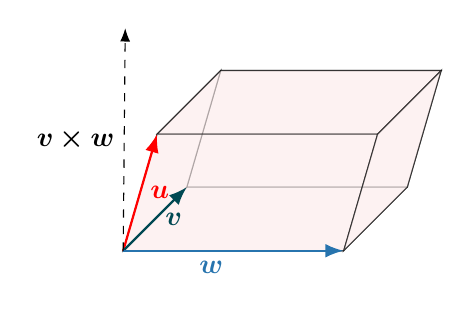
\begin{tikzpicture}[scale=.7]
			\newcommand{\Depth}{3}
			\newcommand{\Height}{2.5}
			\newcommand{\Width}{4}
			\newcommand{\Skew}{1}
			
			\coordinate (a) at (0,0,0);
			\coordinate (b) at (\Width,0,0);
			\coordinate (c) at (\Width + \Skew,\Height,\Skew);
			\coordinate (d) at (\Skew,\Height,\Skew);
			\coordinate (e) at (0,0,\Depth);
			\coordinate (f) at (\Width,0,\Depth);
			\coordinate (g) at (\Width + \Skew,\Height,\Depth + \Skew);
			\coordinate (h) at (\Skew,\Height,\Depth + \Skew);
			
			\coordinate (i) at (\Skew,5,\Depth+ 2.5);
			
			\draw[fill=rosequartz!30,opacity=0.6] (a) -- (b) -- (c) -- (d) -- (a);
			\draw[fill=rosequartz!30,opacity=0.6] (a) -- (e) -- (f) -- (b) -- (a);
			\draw[fill=rosequartz!30,opacity=0.6] (a) -- (d) -- (h) -- (e) -- (a);
			\draw[fill=rosequartz!30,opacity=0.6] (d) -- (c) -- (g) -- (h) -- (d);
			\draw[fill=rosequartz!30,opacity=0.6] (e) -- (f) -- (g) -- (h) -- (e);
			\draw[fill=rosequartz!30,opacity=0.6] (b) -- (c) -- (g) -- (f) -- (b);
			
			\draw[red, thick, -Latex] (e) -- (h) node[midway,right] {$\bm{u}$};
			\draw[megreen, thick, -Latex] (e) -- (a) node[midway,right] {$\bm{v}$};
			\draw[UCLAblue, thick, -Latex] (e) -- (f) node[midway, below left] {$\bm{w}$};
			
			\draw[dashed, -Latex] (e) -- (i) node[midway, left] {$\bm{v \times w}$};
			
			% \node[place, label=below right:{(4,2,1)}] at (a) {};
			% \node[place, label=right:{(1,7,1)}] at (b) {};
			% \node[place, label=above:{(2,9,7)}] at (c) {};
			% \node[place, label=above:{(5,4,7)}] at (d) {};
			% \node[place, label=below:{(8,1,0)}] at (e) {};
			% \node[place, label=below:{(5,6,0)}] at (f) {};
			% \node[place, label=above left:{(6,8,6)}] at (g) {};
			% \node[place, label=left:{(9,3,6)}]  at (h) {};
			
		\end{tikzpicture}
		
	\end{center}
	
	
	
	\begin{center}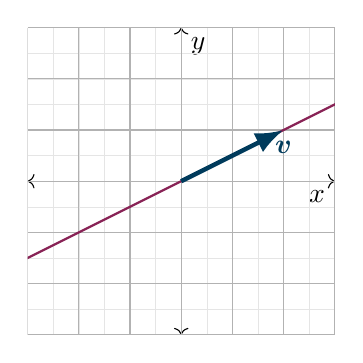
\begin{tikzpicture}[scale=.65]
			\pgfmathsetmacro{\entrya}{2}
			\pgfmathsetmacro{\entryb}{1}
			\clip (-3,-3) rectangle (3,3);
			% Axes
			\draw [<->] (-3,0) -- (3,0) node [below left] {$x$};
			\draw [<->] (0,-3) -- (0,3) node [below right] {$y$};
			%grid
			\draw[step=0.5cm, gray!20!white, very thin] (-3,-3) grid (3,3);
			\draw[step=1cm, gray!60!white, thin] (-3,-3) grid (3,3);
			
			\draw[domain=-3:3,smooth,variable=\t,color=mered, thick]plot (\entrya*\t,\entryb*\t);			
			\draw[color=UCLAdark, ultra thick, -Latex] (0, 0) -- (\entrya,\entryb) node[below]{$\bm{v}$};
			
			
		\end{tikzpicture}
	\end{center}
	
	
	\begin{center}
		\tdplotsetmaincoords{105}{-30}
		\begin{tikzpicture}[tdplot_main_coords,scale=.5]
			\tdplotsetrotatedcoords{00}{30}{0}
			\begin{scope}[tdplot_rotated_coords]
				\draw[color=mered, thick] (0,0,-3) -- (0,0,3);				
				\draw[ultra thick,-Latex,color=UCLAdark] (0,0,0) coordinate (O) -- (0,0,3) node[right]{$\bm{v}$};
			\end{scope}
			\pgfmathsetmacro{\Radius}{1.5}
			\draw[-stealth]  (O)-- (2.5*\Radius,0,0) node[pos=1.15] {$y$};
			\draw[-stealth] (O) -- (0,3.5*\Radius,0) node[pos=1.15] {$x$};
			\draw[-stealth] (O) -- (0,0,2.5*\Radius) node[pos=1.05] {$z$};
		\end{tikzpicture} 
	\end{center}
	
\end{document}